\documentclass[14pt,titlepage, a4paper]{extarticle}
\usepackage{tikz}
\usepackage{pgfplots}
\usetikzlibrary{shapes.geometric, arrows, positioning}
\usepackage{multicol}
\usepackage{minted}
\usepackage[a4paper, margin=0.5in]{geometry}
% tikz styling
\tikzstyle{block} = [rectangle, 
			draw, 
			rounded corners, 
			text centered, 
			minimum height = 2em]
\tikzstyle{rect} = [rectangle, 
			draw, 
			text centered, 
			minimum height = 2em]
\tikzstyle{nrect} = [rectangle, 
			text centered, 
			minimum height = 2em]
\tikzstyle{line} = [draw, -latex']
\tikzstyle{cloud} = [draw, ellipse, minimum height=2em]

\title{Networks Lab Report\\Assignment 3}
\author{Md Sahil\\BCSE III\\Roll-001710501029}
\date{}

\begin{document}

{\maketitle}

\section{Objective}
To implement 1-persistent, non-persistent and p-persistent CSMA techniques.

\section{Design and Implementation}

\subsection{Program structure}
The implementation is done using sockets.
The clients and server communicate with each other using sockets.
Listening on the channel is done through a separate 
thread (for both client and server).
There can be multiple client instances. All the clients are connected to the
central server. The cental server holds the channel(a buffer).


\subsubsection{The Server class}
The server class instance acts as a medium to connect two clients. 
Whenever the server is starts listening and accepting client socket
connections. Each time a client connection is made, its control is
passed on to the client handler thread. The client handler thread then 
listens for incoming frames from the assigned client socket.
The server also maintains a list of mappings of clients with port 
numbers and client addresses. When ever a client tries to connect to a server. 
The server maps the port number with the client address.
When a client tries to sent messages to another client, the server checks the
destination address of the message, finds the port mapped to the address
and forwards the message to the destination client.
The server holds the incomming messages in a buffer, which acts as the channel here.
When ever a new packet arrives and the buffer is non empty, a collision is registered.
\par\null\par
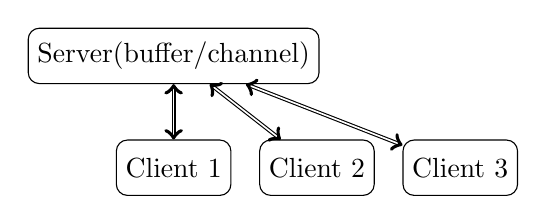
\begin{tikzpicture}[node distance = 1em, auto]
	\node [block] (server) {Server(buffer/channel)};
	\node [block, below=2em of server] (client1) {Client 1};
	\node [block, right=of client1] (client2) {Client 2};
	\node [block, right=of client2] (client3) {Client 3};
	\draw [double,<->] (server) -- (client1);
	\draw [double,<->] (server) -- (client2);
	\draw [double,<->] (server) -- (client3);
\end{tikzpicture}

\subsubsection{The Client class}
The instances of Client class acts as stations. It has 3 functions 
\emph{onePersistent()}, \emph{nonPersistent()} and \emph{pPersistent()}.
Each function implements its corresponding CSMA technique.

\par\null\par
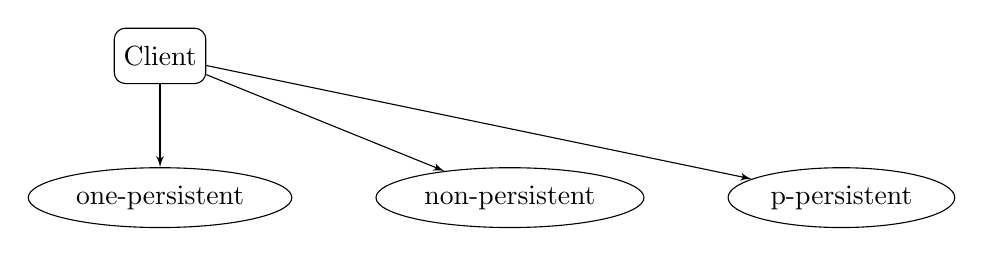
\begin{tikzpicture}[node distance = 3em, auto]
	\node [block] (clientClass) {Client};
	\node [cloud, below=of clientClass] (one) {one-persistent};
	\path [line] (clientClass) -- (one);
	\node [cloud, right=of one] (non) {non-persistent};
	\path [line] (clientClass) -- (non);
	\node [cloud, right=of non] (p) {p-persistent};
	\path [line] (clientClass) -- (p);
\end{tikzpicture}



\section{Code snippets}
\subsection{Server}
\input{./Server.tex}
\subsection{Client}
\input{./Client.tex}

\section{Results}
Observations have been taken by sending 100 packets from each station.

\begin{table}[!ht]
	\caption{With 2 stations}
	\bigskip
	\begin{tabular}{|l|l|l|l|l|l|l|}
		\hline
		&
		\multicolumn{2}{|l|}{one-persisent} & 
		\multicolumn{2}{|l|}{non-persisent} & 
		\multicolumn{2}{|l|}{p-persisent}\\
		\hline
		Sender &
		Throughput & Efficiency & 
		Throughput & Efficiency & 
		Throughput & Efficiency \\ 
		\hline
		1 & 
		0.9459 & 0.72 &
		0.2996 & 1.00 & 
		0.2504 & 1.00\\
		\hline
		2 &
		0.9458 & 0.62 & 
		0.2710 & 0.99 
		& 0.2465 & 0.99\\
		\hline
	\end{tabular}
\end{table}

\begin{table}[!ht]
	\caption{With 3 stations}
	\bigskip
	\begin{tabular}{|l|l|l|l|l|l|l|}
		\hline
		&
		\multicolumn{2}{|l|}{one-persisent} & 
		\multicolumn{2}{|l|}{non-persisent} & 
		\multicolumn{2}{|l|}{p-persisent}\\
		\hline
		Sender &
		Throughput & Efficiency & 
		Throughput & Efficiency & 
		Throughput & Efficiency \\ 
		\hline
		1 &
		0.8748 & 0.46 &
		0.2658 & 0.99 &
		0.1804 & 1.00\\
		\hline
		2 &
		0.8663 & 0.49 & 
		0.2490 & 1.00 &
		0.1711 & 0.99\\
		\hline
		3 &
		0.8505 & 0.52 &
		0.2342 & 0.99 &
		0.1697 & 0.99\\
		\hline
	\end{tabular}
\end{table}

\begin{table}[!ht]
	\caption{With 4 stations}
	\bigskip
	\begin{tabular}{|l|l|l|l|l|l|l|}
		\hline
		&
		\multicolumn{2}{|l|}{one-persisent} & 
		\multicolumn{2}{|l|}{non-persisent} & 
		\multicolumn{2}{|l|}{p-persisent}\\
		\hline
		Sender &
		Throughput & Efficiency & 
		Throughput & Efficiency & 
		Throughput & Efficiency \\ 
		\hline
		1 &
		0.6447 & 0.35 &
		0.1980 & 0.93 & 
		0.1841 & 0.98\\
		\hline
		2 & 
		0.6196 & 0.34 &
		0.1962 & 0.97 & 
		0.1712 & 0.99\\
		\hline
		3 &
		0.6197 & 0.47 &
		0.1891 & 0.95 & 
		0.1816 & 0.99\\
		\hline
		4 &
		0.6157 & 0.37 & 
		0.1852 & 0.95 & 
		0.1555 & 0.97\\
		\hline
	\end{tabular}
\end{table}

\subsection{One-persisent}
\begin{tikzpicture}
\begin{axis}[name=oneeff,
	xlabel = {no of stations},
	ylabel = {Efficiency},
	ymin = 0,
	ymax = 1,
	xtick = {2,3,4}] 
	\addplot[color=red, nodes near coords, mark=x] 
	table{./data/1_efficiency};
\end{axis}	
\end{tikzpicture}
\null
\begin{tikzpicture}
\begin{axis}[name=oneput,
	xlabel = {no of stations},
	ylabel = {Throughput}, 
	xtick = {2,3,4}] 
	\addplot[color=red, nodes near coords, mark=x] 
	table{./data/1_throughput};
\end{axis}	
\end{tikzpicture}

\subsection{Non-persisent}
\begin{tikzpicture}
\begin{axis}[name=oneeff,
	xlabel = {no of stations},
	ylabel = {Efficiency},
	ymin = 0,
	xtick = {2,3,4}] 
	\addplot[color=red, nodes near coords, mark=x] 
	table{./data/n_efficiency};
\end{axis}	
\end{tikzpicture}
\null
\begin{tikzpicture}
\begin{axis}[name=oneput,
	xlabel = {no of stations},
	ylabel = {Throughput}, 
	xtick = {2,3,4}] 
	\addplot[color=red, nodes near coords, mark=x] 
	table{./data/n_throughput};
\end{axis}	
\end{tikzpicture}

\subsection{p-persisent}
For The following graphs we keep the value of \emph{p} at 0.5 and
vary the number of stations.
\\

\noindent
\begin{tikzpicture}
\begin{axis}[name=oneeff,
	xlabel = {no of stations},
	ylabel = {Efficiency},
	ymin = 0,
	xtick = {2,3,4}] 
	\addplot[color=red, nodes near coords, mark=x] 
	table{./data/p_efficiency};
\end{axis}	
\end{tikzpicture}
\null
\begin{tikzpicture}
\begin{axis}[name=oneput,
	xlabel = {no of stations},
	ylabel = {Throughput}, 
	xtick = {2,3,4}] 
	\addplot[color=red, nodes near coords, mark=x] 
	table{./data/p_throughput};
\end{axis}	
\end{tikzpicture}

\noindent
For the following graphs we keep the number of stations fixed at 3 and
vary the value of \emph{p}.
\\
\begin{tikzpicture}
\begin{axis}[name=oneeff,
	xlabel = {p},
	ylabel = {Efficiency},
	ymin = 0,
	xtick = {0.2,0.5,0.8}] 
	\addplot[color=red, nodes near coords, mark=x] 
	table{./data/pp_efficiency};
\end{axis}	
\end{tikzpicture}
\null
\begin{tikzpicture}
\begin{axis}[name=oneput,
	xlabel = {p},
	ylabel = {Throughput}, 
	xtick = {0.2,0.5,0.8}] 
	\addplot[color=red, nodes near coords, mark=x] 
	table{./data/pp_throughput};
\end{axis}	
\end{tikzpicture}

\pagebreak
\section{Comments}
\begin{itemize}
		\item The architecture of the code here is identical 
			to the previous assignment. 
		\item I faced some thread scheduling problems.
			For example in certain infinite while loops, adding a blank print statement
			changed the execution.
\end{itemize}

\end{document}
